
% !TEX encoding = UTF-8 Unicode 
% !TEX root = FieldGuide.tex

\subpart{Three (or more) shape parameters}

\Sec{Generalized Beta Distribution}
\label{sec:GenBeta}
\phantomsection
\addcontentsline{toc}{subsection}{~~~~~~~~~~~~Generalized beta} 

The {\bf generalized beta} (beta-power)  distribution~\cite{McDonald1984} is a five parameter,  continuous, univariate, unimodal probability density, with finite or semi infinite support. The functional form in the most straightforward parameterizaton is
\begin{align}
\label{GenBeta}
\opr{GenBeta}&(x\given a,s,\alpha, \gamma,\beta) 
\\    = & 
 \frac{1}{B(\alpha, \gamma)} \Left|\frac{\beta}{s}\Right|
\Left(\frac{x-a}{s} \Right)^{\alpha \beta -1} \Left (1-\Left(\frac{x-a}{s}\Right)^\beta\Right)^{\gamma -1}
\notag
\checked
\\
& \text{for } x,\ a,\ \theta,\ \alpha,\ \gamma,\ \beta\  \text{in } \mathbb{R}, 
\notag
\\ & \alpha>0, \  \gamma >0
\notag
 \\ \text{ support } \checked & x \in [a,a+s], s>0,\ \beta>0 \notag
  \\  &  x\in[a+s,a], s<0,\ \beta>0 
 \notag 
 \\  \notag  &  x\in[a+s,+\infty], s>0,\ \beta<0 
 \\  \notag  &  x\in[-\infty,a+s], s<0,\ \beta<0 
\notag
\end{align}
The generalized beta distribution arises as the Weibullization of the standard beta distribution, $x\rightarrow (\tfrac{x-a}{s})^{\beta}$, and as the order statistics of the power function distribution~\eqref{PowerFn}. The parameters consist of a location parameter $a$, shape parameter~$s$, Weibull power parameter $\beta$, and two shape parameters~$\alpha$ and~$\gamma$.




\begin{table*}[tp!]
%\addcontentsline{toc}{subsection}{Beta} 
\begin{center}
\caption[Generalized beta distributions -- Special cases] {Special cases of generalized beta}
\label{GenBetaTable}
~\\

%Note: Power func special cases go under power function.
{\renewcommand{\arraystretch}{1.25} 
\begin{tabular}{llccccc@{\extracolsep{5pt}} l}
\eqref{GenBeta} &generalized beta & $a$ & $s$ & $\alpha$ & $\gamma$ & $\beta$ &
\\ \hline
\eqref{Kumaraswamy} & Kumaraswamy 		& . & . & 1 & . & . &\\
\\
\eqref{Beta} & beta				& .   & .& . & . & 1 &   \\
\eqref{StdBeta}  & standard beta 		& 0  & 1 & . & . & 1 &\\
\eqref{Beta} & beta, U shaped 		& . & . & $<\!\!1$ & $<\!\!1$ & 1 &\\
\eqref{Beta} & beta, J shaped 		& .  & . & . & . & 1 & {\small $(\alpha$-$1)(\gamma$-$1) \leq 0$} \\
\eqref{CentralBeta} & central-beta  		&  .  & . & $\alpha$ & $\alpha$ & 1 & \\
\eqref{Arcsine} & arcsine 				& .  & . & $\frac{1}{2}$ & $\frac{1}{2}$ & 1 & \\
%\eqref{CentralArcsine}& central arcsine 		& -$b$  & $2b$ & $\frac{1}{2}$ & $\frac{1}{2}$ & 1 & \\
\eqref{Semicircle}& semicircle 		& -$b$  & $2b$ & $1\frac{1}{2}$ & $1\frac{1}{2}$ & 1 & \\
\eqref{Epanechnikov}&Epanechnikov & . & . & 2 & 2 & 1 \\ 
\eqref{Biweight}&biweight & . & . & 3 & 3 & 1 \\ 
\eqref{Triweight}&triweight & . & . & 4 & 4 & 1 \\ 
%\eqref{PowerFn} & power function		& . & . & . & 1 & 1& \\
%\eqref{PowerFn} & reciprocal		& . & . & 0 & 1 & 1& \\
%\eqref{PowerFn} & Pearson type VIII 		& 0 & . &  $<\!\!1$ & 1& 1&\\
%\eqref{PowerFn} & Pearson type IX 		& 0 & .  & $>\!\!1$ & 1 & 1&\\
\eqref{PearsonXII}  & Pearson  XII  		& . & . & . &  2-$\alpha$&1& $\alpha<2$ \\
%\eqref{Wedge} & wedge			& . & . & 2 & 1 & 1 &\\
\\
\eqref{BetaPrime} & beta-prime			& . & . & . & . & -1 \\
\eqref{PowerFn} & power function		& . & . & 1 & 1 & . & \\
\eqref{Uniform} & uniform			& . & . & 1 & 1 & 1 &\\
\eqref{Uniform} & standard uniform		& 0 & 1 & 1 & 1 & 1 &\\
%\\
%& \underline{Limits}
%\\
%\eqref{UnitGamma} & unit gamma &                         . & . & $\alpha$ &.&  $\tfrac{\delta}{\alpha}$ & $\lim_{\alpha\rightarrow\infty }$ \\ 
%\eqref{Amoroso} & Amoroso			& . & $\theta \gamma^{\frac{1}{\beta}}$& . & $\gamma$ & . &    $\lim_{\gamma\rightarrow\infty}$ \\
%\eqref{BetaExp} & beta exp.			& ${\pLoc\text{-}\beta\pScale}$ & $\beta\pScale$ & . & . &$\beta$ &    $\lim_{\beta\rightarrow\infty}$ \\
\end{tabular} 
}
\end{center}
\end{table*}


% !TEX encoding = UTF-8 Unicode 
% !TEX root = FieldGuide.tex

\begin{table*}[tp]
\caption[Generalized beta distribution-- Properties]{Properties of the generalized beta distribution}
 \begin{align*}
 \text{\hyperref[PropertiesSec]{Properties}}  \quad& \\
\text{name} \quad & \text{GenBeta}(x\given a,s,\alpha, \gamma,\beta) 
\\
\text{PDF}\quad &   \frac{1}{B(\alpha, \gamma)} \left|\frac{\beta}{s}\right|
\left(\frac{x-a}{s} \right)^{\alpha \beta -1} \left(1-\left(\frac{x-a}{s}\right)^\beta\right)^{\gamma -1}
\checked
\hspace{-8em}
\\
\text{CDF / CCDF} \quad  &   \frac{B\left( \alpha,\gamma; (\tfrac{x-a}{s})^\beta  \right)}{B(\alpha,\gamma)}
\checked
% McDonald1984 table 3.1 GB1
& \tfrac{\beta}{s} >0 \,\big/ \, \tfrac{\beta}{s} <0
\\ & \quad = I\left(  \alpha,\gamma; (\tfrac{x-a}{s})^\beta \right) \checked
\\ 
\text{parameters}\quad &   a,\ s,\ \alpha,\ \gamma,\ \beta, \text{ in } \Real, \\ &  \alpha,\gamma\geq0
\\
\text{support} \quad 
&   \ x \in [a,a+s],  \quad & 0<s,\ 0<\beta  \checked
 \\ 	 		 & \ x\in[a+s,a],  \quad & s<0,\ 0<\beta   \checked
 \\  			 & \ x\in[a+s,+\infty], \quad  & 0<s,\ \beta<0  \checked
 \\  			& \ x\in[-\infty,a+s], \quad & s<0,\ \beta<0 \checked
\\
%\text{median} \quad  &  \cdots
%\\
%\text{mode} \quad  & \cdots
%\\
\text{mean} \quad  &   a+ \frac{s B(\alpha+\tfrac{1}{\beta},\gamma) }{B(\alpha,\gamma)}  \quad & \alpha+\tfrac{1}{\beta} >0
\checked
\\
\text{variance} \quad  & \frac{s^2 B(\alpha+\tfrac{2}{\beta},\gamma) }{B(\alpha,\gamma)} -\frac{s^2 B(\alpha+\tfrac{1}{\beta},\gamma)^2 }{B(\alpha,\gamma)^2} \checked
\\
\text{skew} \quad  &   \text{not simple}
\\
\text{kurtosis} \quad  &   \text{not simple}
\\
% \text{entropy} \quad  & \cdots
% \\
\text{MGF} \quad  &  \text{none} % Can't exist because beta mgf doesn't exist
\\
% \text{CF} \quad  &  \cdots
% \\
E(X^h) \quad & \frac{s^h B(\alpha+\tfrac{h}{\beta},\gamma) }{B(\alpha,\gamma)}  \qquad  & \!\!a=0,\ \alpha+\tfrac{h}{\beta} >0
\ \text{\cite{McDonald1984}} \checked
%{Normalize style, use similar style in beta properties table.}
\end{align*}
\end{table*}



\SSec{Special Cases}

The beta distribution ($\beta$=1) and specializations are described in \secref{sec:Beta}.

\dist{Kumaraswamy} (minimax) distribution~\cite{Kumaraswamy1980, Leemis2008, Jones2009}:
\begin{align}
\label{Kumaraswamy}
\opr{Kumaraswamy}(x\given a,s,\gamma,\beta) &= \gamma \Left|\frac{\beta}{s}\Right| \Left(\frac{x-a}{s}\Right)^{\beta-1} \Left(1-\Left(\frac{x-a}{s}\Right)^{\beta}\Right)^{\gamma-1} \checked
\\
&= \opr{GenBeta}(x\given a,s,1,\gamma,\beta)  \notag \checked
\end{align}
Proposed as an alternative to the beta distribution for modeling bounded variables, since the cumulative distribution function has a simple closed form, 
\[\op{KumaraswamyCDF}(x\given 0, 1, \gamma,\beta) = 1- (1-x^{\beta})^\gamma. \checked \notag\]


\begin{figure}[tp!]
\begin{center}
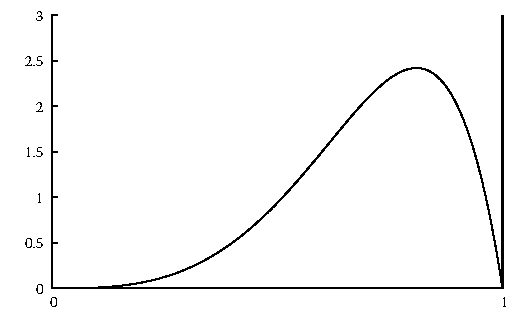
\includegraphics[width=\textwidth]{pdfKumaraswamy}
\end{center}
\caption[Kumaraswamy distribution]{A Kumaraswamy distribution, $\opr{Kumaraswamy}(0, 1, 2, 4)$}
\end{figure}


\SSec{Interrelations}

The generalized beta distribution describes the order statistics of a power function  distribution \eqref{PowerFn}.
\begin{align*}
\opr{OrderStatistic}_{\opr{PowerFn}(a,s,\beta)} &(x \given \alpha, \gamma) = \opr{GenBeta}(x\given a, s, \alpha,\gamma, \beta) 
\checked
\end{align*}
Conversely, the power function \eqref{PowerFn} distribution is a special case of the generalized beta distribution. 
\begin{align*}
\opr{GenBeta}(x\given a, s, 1, 1,\beta) & = \opr{PowerFn}(x\given a,s,\beta)  \checked
\notag
\end{align*}

Setting $\beta=1$ yields the beta  distribution \eqref{Beta}, 
\[
\opr{GenBeta}(x\given a,s,\alpha, \gamma,1) = \opr{Beta}(x\given a,s,\alpha,\gamma) \ , \checked
\notag
\]
and setting $\beta=-1$ yields the beta prime (or inverse beta) distribution \eqref{BetaPrime},  
\[
\opr{GenBeta}(x\given a,s,\alpha, \gamma,-1) = \opr{BetaPrime}(x\given a+s,s,\gamma,\alpha) \ . \checked
\notag
\]
The beta \secref{sec:Beta} and beta prime \secref{sec:BetaPrime} distributions have many named special cases, see tables~\ref{GenBetaTable} and \ref{GenBetaPrimeTable}.


The unit gamma distribution~\eqref{UnitGamma} arises in the limit $\lim_{\beta\rightarrow0}$ with $\alpha\beta=\text{constant}$,
\[
 \lim_{\beta\rightarrow0 } \opr{GenBeta}(x\given a,s,\tfrac{\delta}{\beta}, \gamma,\beta)  = \opr{UnitGamma}(x\given a, s, \gamma,\delta) \ . \checked
 \notag
\]
In the  limit $\gamma\rightarrow\infty$ (or equivalently $\alpha\rightarrow\infty$) we obtain the Amoroso distribution \eqref{Amoroso} with semi-infinite support, the parent of the gamma distribution family~\cite{McDonald1984},
\[
\lim_{\gamma\rightarrow\infty} \opr{GenBeta}(x\given a, \theta \gamma^{\frac{1}{\beta}} ,\alpha, \gamma, \beta ) = \opr{Amoroso}(x\given a,\theta,\alpha, \beta) \ . \checked
\notag
\]
The limit  $\lim_{\beta\rightarrow+\infty }$ yields the beta-exponential distribution~\eqref{BetaExp}
\[
 \lim_{\beta\rightarrow+\infty } \opr{GenBeta}(x\given \pLoc+\beta\lambda,-\beta\pScale,\alpha,\gamma,\beta) = \opr{BetaExp}(x\given \pLoc,\pScale,\alpha, \gamma) \checked
\ .
\notag
\]




